% Options for packages loaded elsewhere
\PassOptionsToPackage{unicode}{hyperref}
\PassOptionsToPackage{hyphens}{url}
%
\documentclass[
]{article}
\usepackage{amsmath,amssymb}
\usepackage{iftex}
\ifPDFTeX
  \usepackage[T1]{fontenc}
  \usepackage[utf8]{inputenc}
  \usepackage{textcomp} % provide euro and other symbols
\else % if luatex or xetex
  \usepackage{unicode-math} % this also loads fontspec
  \defaultfontfeatures{Scale=MatchLowercase}
  \defaultfontfeatures[\rmfamily]{Ligatures=TeX,Scale=1}
\fi
\usepackage{lmodern}
\ifPDFTeX\else
  % xetex/luatex font selection
\fi
% Use upquote if available, for straight quotes in verbatim environments
\IfFileExists{upquote.sty}{\usepackage{upquote}}{}
\IfFileExists{microtype.sty}{% use microtype if available
  \usepackage[]{microtype}
  \UseMicrotypeSet[protrusion]{basicmath} % disable protrusion for tt fonts
}{}
\makeatletter
\@ifundefined{KOMAClassName}{% if non-KOMA class
  \IfFileExists{parskip.sty}{%
    \usepackage{parskip}
  }{% else
    \setlength{\parindent}{0pt}
    \setlength{\parskip}{6pt plus 2pt minus 1pt}}
}{% if KOMA class
  \KOMAoptions{parskip=half}}
\makeatother
\usepackage{xcolor}
\usepackage[margin=2.54cm]{geometry}
\usepackage{color}
\usepackage{fancyvrb}
\newcommand{\VerbBar}{|}
\newcommand{\VERB}{\Verb[commandchars=\\\{\}]}
\DefineVerbatimEnvironment{Highlighting}{Verbatim}{commandchars=\\\{\}}
% Add ',fontsize=\small' for more characters per line
\usepackage{framed}
\definecolor{shadecolor}{RGB}{248,248,248}
\newenvironment{Shaded}{\begin{snugshade}}{\end{snugshade}}
\newcommand{\AlertTok}[1]{\textcolor[rgb]{0.94,0.16,0.16}{#1}}
\newcommand{\AnnotationTok}[1]{\textcolor[rgb]{0.56,0.35,0.01}{\textbf{\textit{#1}}}}
\newcommand{\AttributeTok}[1]{\textcolor[rgb]{0.13,0.29,0.53}{#1}}
\newcommand{\BaseNTok}[1]{\textcolor[rgb]{0.00,0.00,0.81}{#1}}
\newcommand{\BuiltInTok}[1]{#1}
\newcommand{\CharTok}[1]{\textcolor[rgb]{0.31,0.60,0.02}{#1}}
\newcommand{\CommentTok}[1]{\textcolor[rgb]{0.56,0.35,0.01}{\textit{#1}}}
\newcommand{\CommentVarTok}[1]{\textcolor[rgb]{0.56,0.35,0.01}{\textbf{\textit{#1}}}}
\newcommand{\ConstantTok}[1]{\textcolor[rgb]{0.56,0.35,0.01}{#1}}
\newcommand{\ControlFlowTok}[1]{\textcolor[rgb]{0.13,0.29,0.53}{\textbf{#1}}}
\newcommand{\DataTypeTok}[1]{\textcolor[rgb]{0.13,0.29,0.53}{#1}}
\newcommand{\DecValTok}[1]{\textcolor[rgb]{0.00,0.00,0.81}{#1}}
\newcommand{\DocumentationTok}[1]{\textcolor[rgb]{0.56,0.35,0.01}{\textbf{\textit{#1}}}}
\newcommand{\ErrorTok}[1]{\textcolor[rgb]{0.64,0.00,0.00}{\textbf{#1}}}
\newcommand{\ExtensionTok}[1]{#1}
\newcommand{\FloatTok}[1]{\textcolor[rgb]{0.00,0.00,0.81}{#1}}
\newcommand{\FunctionTok}[1]{\textcolor[rgb]{0.13,0.29,0.53}{\textbf{#1}}}
\newcommand{\ImportTok}[1]{#1}
\newcommand{\InformationTok}[1]{\textcolor[rgb]{0.56,0.35,0.01}{\textbf{\textit{#1}}}}
\newcommand{\KeywordTok}[1]{\textcolor[rgb]{0.13,0.29,0.53}{\textbf{#1}}}
\newcommand{\NormalTok}[1]{#1}
\newcommand{\OperatorTok}[1]{\textcolor[rgb]{0.81,0.36,0.00}{\textbf{#1}}}
\newcommand{\OtherTok}[1]{\textcolor[rgb]{0.56,0.35,0.01}{#1}}
\newcommand{\PreprocessorTok}[1]{\textcolor[rgb]{0.56,0.35,0.01}{\textit{#1}}}
\newcommand{\RegionMarkerTok}[1]{#1}
\newcommand{\SpecialCharTok}[1]{\textcolor[rgb]{0.81,0.36,0.00}{\textbf{#1}}}
\newcommand{\SpecialStringTok}[1]{\textcolor[rgb]{0.31,0.60,0.02}{#1}}
\newcommand{\StringTok}[1]{\textcolor[rgb]{0.31,0.60,0.02}{#1}}
\newcommand{\VariableTok}[1]{\textcolor[rgb]{0.00,0.00,0.00}{#1}}
\newcommand{\VerbatimStringTok}[1]{\textcolor[rgb]{0.31,0.60,0.02}{#1}}
\newcommand{\WarningTok}[1]{\textcolor[rgb]{0.56,0.35,0.01}{\textbf{\textit{#1}}}}
\usepackage{graphicx}
\makeatletter
\def\maxwidth{\ifdim\Gin@nat@width>\linewidth\linewidth\else\Gin@nat@width\fi}
\def\maxheight{\ifdim\Gin@nat@height>\textheight\textheight\else\Gin@nat@height\fi}
\makeatother
% Scale images if necessary, so that they will not overflow the page
% margins by default, and it is still possible to overwrite the defaults
% using explicit options in \includegraphics[width, height, ...]{}
\setkeys{Gin}{width=\maxwidth,height=\maxheight,keepaspectratio}
% Set default figure placement to htbp
\makeatletter
\def\fps@figure{htbp}
\makeatother
\setlength{\emergencystretch}{3em} % prevent overfull lines
\providecommand{\tightlist}{%
  \setlength{\itemsep}{0pt}\setlength{\parskip}{0pt}}
\setcounter{secnumdepth}{-\maxdimen} % remove section numbering
\ifLuaTeX
  \usepackage{selnolig}  % disable illegal ligatures
\fi
\usepackage{bookmark}
\IfFileExists{xurl.sty}{\usepackage{xurl}}{} % add URL line breaks if available
\urlstyle{same}
\hypersetup{
  pdftitle={Assignment 5: Data Visualization},
  pdfauthor={Shuer Li},
  hidelinks,
  pdfcreator={LaTeX via pandoc}}

\title{Assignment 5: Data Visualization}
\author{Shuer Li}
\date{Fall 2025}

\begin{document}
\maketitle

\subsection{OVERVIEW}\label{overview}

This exercise accompanies the lessons in Environmental Data Analytics on
Data Visualization

\subsection{Directions}\label{directions}

\begin{enumerate}
\def\labelenumi{\arabic{enumi}.}
\tightlist
\item
  Rename this file
  \texttt{\textless{}FirstLast\textgreater{}\_A05\_DataVisualization.Rmd}
  (replacing \texttt{\textless{}FirstLast\textgreater{}} with your first
  and last name).
\item
  Change ``Student Name'' on line 3 (above) with your name.
\item
  Work through the steps, \textbf{creating code and output} that fulfill
  each instruction.
\item
  Be sure your code is tidy; use line breaks to ensure your code fits in
  the knitted output.
\item
  Be sure to \textbf{answer the questions} in this assignment document.
\item
  When you have completed the assignment, \textbf{Knit} the text and
  code into a single PDF file.
\end{enumerate}

\begin{center}\rule{0.5\linewidth}{0.5pt}\end{center}

\subsection{Set up your session}\label{set-up-your-session}

\begin{enumerate}
\def\labelenumi{\arabic{enumi}.}
\item
  Set up your session. Load the tidyverse, here \& cowplot packages, and
  verify your home directory. Read in the NTL-LTER processed data files
  for nutrients and chemistry/physics for Peter and Paul Lakes (use the
  tidy
  \texttt{NTL-LTER\_Lake\_Chemistry\_Nutrients\_PeterPaul\_Processed.csv}
  version in the Processed\_KEY folder) and the processed data file for
  the Niwot Ridge litter dataset (use the
  \texttt{NEON\_NIWO\_Litter\_mass\_trap\_Processed.csv} version, again
  from the Processed\_KEY folder).
\item
  Make sure R is reading dates as date format; if not change the format
  to date.
\end{enumerate}

\begin{Shaded}
\begin{Highlighting}[]
\CommentTok{\#1 Load necessary packages}
\FunctionTok{library}\NormalTok{(tidyverse)}
\end{Highlighting}
\end{Shaded}

\begin{verbatim}
## -- Attaching core tidyverse packages ------------------------ tidyverse 2.0.0 --
## v dplyr     1.1.4     v readr     2.1.5
## v forcats   1.0.0     v stringr   1.5.1
## v ggplot2   4.0.0     v tibble    3.2.1
## v lubridate 1.9.4     v tidyr     1.3.1
## v purrr     1.0.2     
## -- Conflicts ------------------------------------------ tidyverse_conflicts() --
## x dplyr::filter() masks stats::filter()
## x dplyr::lag()    masks stats::lag()
## i Use the conflicted package (<http://conflicted.r-lib.org/>) to force all conflicts to become errors
\end{verbatim}

\begin{Shaded}
\begin{Highlighting}[]
\FunctionTok{library}\NormalTok{(here)}
\end{Highlighting}
\end{Shaded}

\begin{verbatim}
## here() starts at /home/guest/EDE_Fall2025
\end{verbatim}

\begin{Shaded}
\begin{Highlighting}[]
\FunctionTok{library}\NormalTok{(cowplot)}
\end{Highlighting}
\end{Shaded}

\begin{verbatim}
## 
## Attaching package: 'cowplot'
## 
## The following object is masked from 'package:lubridate':
## 
##     stamp
\end{verbatim}

\begin{Shaded}
\begin{Highlighting}[]
\CommentTok{\# Verify the working directory}
\FunctionTok{here}\NormalTok{()}
\end{Highlighting}
\end{Shaded}

\begin{verbatim}
## [1] "/home/guest/EDE_Fall2025"
\end{verbatim}

\begin{Shaded}
\begin{Highlighting}[]
\CommentTok{\# Define the processed data folder}
\NormalTok{processed\_data }\OtherTok{\textless{}{-}} \FunctionTok{here}\NormalTok{(}\StringTok{"Data/Processed\_KEY"}\NormalTok{)}

\CommentTok{\# Read the Peter and Paul Lakes data}
\NormalTok{PeterPaul.chem.nutrients }\OtherTok{\textless{}{-}} \FunctionTok{read.csv}\NormalTok{(}
  \FunctionTok{here}\NormalTok{(processed\_data, }\StringTok{"NTL{-}LTER\_Lake\_Chemistry\_Nutrients\_PeterPaul\_Processed.csv"}\NormalTok{),}
  \AttributeTok{stringsAsFactors =} \ConstantTok{TRUE}\NormalTok{)}

\CommentTok{\# Read the Niwot Ridge litter dataset}
\NormalTok{NIWO.litter }\OtherTok{\textless{}{-}} \FunctionTok{read.csv}\NormalTok{(}
  \FunctionTok{here}\NormalTok{(processed\_data, }\StringTok{"NEON\_NIWO\_Litter\_mass\_trap\_Processed.csv"}\NormalTok{),}
  \AttributeTok{stringsAsFactors =} \ConstantTok{TRUE}\NormalTok{)}

\CommentTok{\#2 Check which columns are dates}
\FunctionTok{names}\NormalTok{(PeterPaul.chem.nutrients)}
\end{Highlighting}
\end{Shaded}

\begin{verbatim}
##  [1] "lakename"        "year4"           "daynum"          "month"          
##  [5] "sampledate"      "depth"           "temperature_C"   "dissolvedOxygen"
##  [9] "irradianceWater" "irradianceDeck"  "tn_ug"           "tp_ug"          
## [13] "nh34"            "no23"            "po4"
\end{verbatim}

\begin{Shaded}
\begin{Highlighting}[]
\FunctionTok{names}\NormalTok{(NIWO.litter)}
\end{Highlighting}
\end{Shaded}

\begin{verbatim}
##  [1] "plotID"           "trapID"           "collectDate"      "functionalGroup" 
##  [5] "dryMass"          "qaDryMass"        "subplotID"        "decimalLatitude" 
##  [9] "decimalLongitude" "elevation"        "nlcdClass"        "plotType"        
## [13] "geodeticDatum"
\end{verbatim}

\begin{Shaded}
\begin{Highlighting}[]
\CommentTok{\# Convert date columns to proper Date format}
\NormalTok{PeterPaul.chem.nutrients}\SpecialCharTok{$}\NormalTok{sampledate }\OtherTok{\textless{}{-}} \FunctionTok{ymd}\NormalTok{(PeterPaul.chem.nutrients}\SpecialCharTok{$}\NormalTok{sampledate)}
\NormalTok{NIWO.litter}\SpecialCharTok{$}\NormalTok{collectDate }\OtherTok{\textless{}{-}} \FunctionTok{ymd}\NormalTok{(NIWO.litter}\SpecialCharTok{$}\NormalTok{collectDate)}

\CommentTok{\# Verify that conversion was successful}
\FunctionTok{str}\NormalTok{(PeterPaul.chem.nutrients}\SpecialCharTok{$}\NormalTok{sampledate)}
\end{Highlighting}
\end{Shaded}

\begin{verbatim}
##  Date[1:23008], format: "1984-05-27" "1984-05-27" "1984-05-27" "1984-05-27" "1984-05-27" ...
\end{verbatim}

\begin{Shaded}
\begin{Highlighting}[]
\FunctionTok{str}\NormalTok{(NIWO.litter}\SpecialCharTok{$}\NormalTok{collectDate)}
\end{Highlighting}
\end{Shaded}

\begin{verbatim}
##  Date[1:1692], format: "2016-06-16" "2016-06-16" "2016-06-16" "2016-06-16" "2016-06-16" ...
\end{verbatim}

\subsection{Define your theme}\label{define-your-theme}

\begin{enumerate}
\def\labelenumi{\arabic{enumi}.}
\setcounter{enumi}{2}
\tightlist
\item
  Build a theme and set it as your default theme. Customize the look of
  at least two of the following:
\end{enumerate}

\begin{itemize}
\tightlist
\item
  Plot background
\item
  Plot title
\item
  Axis labels
\item
  Axis ticks/gridlines
\item
  Legend
\end{itemize}

\begin{Shaded}
\begin{Highlighting}[]
\CommentTok{\#3 Create a custom theme}
\FunctionTok{library}\NormalTok{(ggthemes)}
\end{Highlighting}
\end{Shaded}

\begin{verbatim}
## 
## Attaching package: 'ggthemes'
\end{verbatim}

\begin{verbatim}
## The following object is masked from 'package:cowplot':
## 
##     theme_map
\end{verbatim}

\begin{Shaded}
\begin{Highlighting}[]
\NormalTok{mytheme }\OtherTok{\textless{}{-}} \FunctionTok{theme\_base}\NormalTok{() }\SpecialCharTok{+}
  \FunctionTok{theme}\NormalTok{(}
    \CommentTok{\# Line color and width}
    \AttributeTok{line =} \FunctionTok{element\_line}\NormalTok{(}
      \AttributeTok{color =} \StringTok{"red"}\NormalTok{,}
      \AttributeTok{linewidth =} \FloatTok{1.2}
\NormalTok{    ),}
    
    \CommentTok{\# Plot background}
    \AttributeTok{plot.background =} \FunctionTok{element\_rect}\NormalTok{(}
      \AttributeTok{fill =} \StringTok{"white"}\NormalTok{,}
      \AttributeTok{color =} \StringTok{"gray85"}
\NormalTok{    ),}
    
    \CommentTok{\# Plot title}
    \AttributeTok{plot.title =} \FunctionTok{element\_text}\NormalTok{(}
      \AttributeTok{face =} \StringTok{"bold"}\NormalTok{,}
      \AttributeTok{size =} \DecValTok{15}\NormalTok{,}
      \AttributeTok{hjust =} \FloatTok{0.5}\NormalTok{,}
      \AttributeTok{color =} \StringTok{"black"}
\NormalTok{    ),}
    
    \CommentTok{\# Axis labels and text}
    \AttributeTok{axis.title =} \FunctionTok{element\_text}\NormalTok{(}
      \AttributeTok{face =} \StringTok{"bold"}\NormalTok{,}
      \AttributeTok{size =} \DecValTok{13}\NormalTok{,}
      \AttributeTok{color =} \StringTok{"black"}
\NormalTok{    ),}
    \AttributeTok{axis.text =} \FunctionTok{element\_text}\NormalTok{(}
      \AttributeTok{size =} \DecValTok{11}\NormalTok{,}
      \AttributeTok{color =} \StringTok{"black"}
\NormalTok{    ),}
    
    \CommentTok{\# Axis gridlines}
    \AttributeTok{panel.grid.major =} \FunctionTok{element\_line}\NormalTok{(}
      \AttributeTok{color =} \StringTok{"gray90"}\NormalTok{,}
      \AttributeTok{linewidth =} \FloatTok{0.4}
\NormalTok{    ),}
    \AttributeTok{panel.grid.minor =} \FunctionTok{element\_blank}\NormalTok{(),}
    
    \CommentTok{\# Legend background and title}
    \AttributeTok{legend.background =} \FunctionTok{element\_rect}\NormalTok{(}
      \AttributeTok{color =} \StringTok{"gray60"}\NormalTok{,}
      \AttributeTok{fill =} \StringTok{"lightyellow"}
\NormalTok{    ),}
    \AttributeTok{legend.title =} \FunctionTok{element\_text}\NormalTok{(}
      \AttributeTok{color =} \StringTok{"blue"}\NormalTok{,}
      \AttributeTok{face =} \StringTok{"bold"}\NormalTok{,}
      \AttributeTok{size =} \DecValTok{12}
\NormalTok{    ),}
    \AttributeTok{legend.text =} \FunctionTok{element\_text}\NormalTok{(}
      \AttributeTok{size =} \DecValTok{11}
\NormalTok{    ),}
    
    \CommentTok{\# Legend position}
    \AttributeTok{legend.position =} \StringTok{"top"}
\NormalTok{  )}

\CommentTok{\# Set as the default theme for all plots}
\FunctionTok{theme\_set}\NormalTok{(mytheme)}
\end{Highlighting}
\end{Shaded}

\subsection{Create graphs}\label{create-graphs}

For numbers 4-7, create ggplot graphs and adjust aesthetics to follow
best practices for data visualization. Ensure your theme, color
palettes, axes, and additional aesthetics are edited accordingly.

\begin{enumerate}
\def\labelenumi{\arabic{enumi}.}
\setcounter{enumi}{3}
\tightlist
\item
  {[}NTL-LTER{]} Plot total phosphorus (\texttt{tp\_ug}) by phosphate
  (\texttt{po4}), with separate aesthetics for Peter and Paul lakes. Add
  line(s) of best fit using the \texttt{lm} method. Adjust your axes to
  hide extreme values (hint: change the limits using \texttt{xlim()}
  and/or \texttt{ylim()}).
\end{enumerate}

\begin{Shaded}
\begin{Highlighting}[]
\CommentTok{\#4 Plot total phosphorus by phosphate}
\CommentTok{\# Add linear regression lines and adjust axis limits to hide outliers}
\FunctionTok{library}\NormalTok{(viridis)}
\end{Highlighting}
\end{Shaded}

\begin{verbatim}
## Loading required package: viridisLite
\end{verbatim}

\begin{Shaded}
\begin{Highlighting}[]
\FunctionTok{ggplot}\NormalTok{(PeterPaul.chem.nutrients, }
       \FunctionTok{aes}\NormalTok{(}\AttributeTok{x =}\NormalTok{ po4, }\AttributeTok{y =}\NormalTok{ tp\_ug, }\AttributeTok{color =}\NormalTok{ lakename)) }\SpecialCharTok{+}
  \FunctionTok{geom\_point}\NormalTok{(}\AttributeTok{alpha =} \FloatTok{0.7}\NormalTok{, }\AttributeTok{size =} \DecValTok{2}\NormalTok{) }\SpecialCharTok{+} \CommentTok{\# scatter points with transparency}
  \FunctionTok{geom\_smooth}\NormalTok{(}\AttributeTok{method =} \StringTok{"lm"}\NormalTok{, }\AttributeTok{se =} \ConstantTok{FALSE}\NormalTok{, }\AttributeTok{linewidth =} \FloatTok{0.8}\NormalTok{) }\SpecialCharTok{+} \CommentTok{\# linear regression lines}
  \FunctionTok{scale\_color\_viridis}\NormalTok{(}\AttributeTok{discrete =} \ConstantTok{TRUE}\NormalTok{, }\AttributeTok{option =} \StringTok{"magma"}\NormalTok{, }\AttributeTok{end =} \FloatTok{0.9}\NormalTok{) }\SpecialCharTok{+} \CommentTok{\# color palette}
  \FunctionTok{xlim}\NormalTok{(}\DecValTok{0}\NormalTok{, }\DecValTok{150}\NormalTok{) }\SpecialCharTok{+} \FunctionTok{ylim}\NormalTok{(}\DecValTok{0}\NormalTok{, }\DecValTok{150}\NormalTok{) }\SpecialCharTok{+} \CommentTok{\# limit axes to remove outliers}
  \FunctionTok{labs}\NormalTok{(}
    \AttributeTok{title =} \StringTok{"Relationship between Total Phosphorus and Phosphate"}\NormalTok{,}
    \AttributeTok{x =} \StringTok{"Phosphate (μg/L)"}\NormalTok{,}
    \AttributeTok{y =} \StringTok{"Total Phosphorus (μg/L)"}\NormalTok{,}
    \AttributeTok{color =} \StringTok{"Lake"}
\NormalTok{  )}
\end{Highlighting}
\end{Shaded}

\begin{verbatim}
## `geom_smooth()` using formula = 'y ~ x'
\end{verbatim}

\begin{verbatim}
## Warning: Removed 21948 rows containing non-finite outside the scale range
## (`stat_smooth()`).
\end{verbatim}

\begin{verbatim}
## Warning: Removed 21948 rows containing missing values or values outside the scale range
## (`geom_point()`).
\end{verbatim}

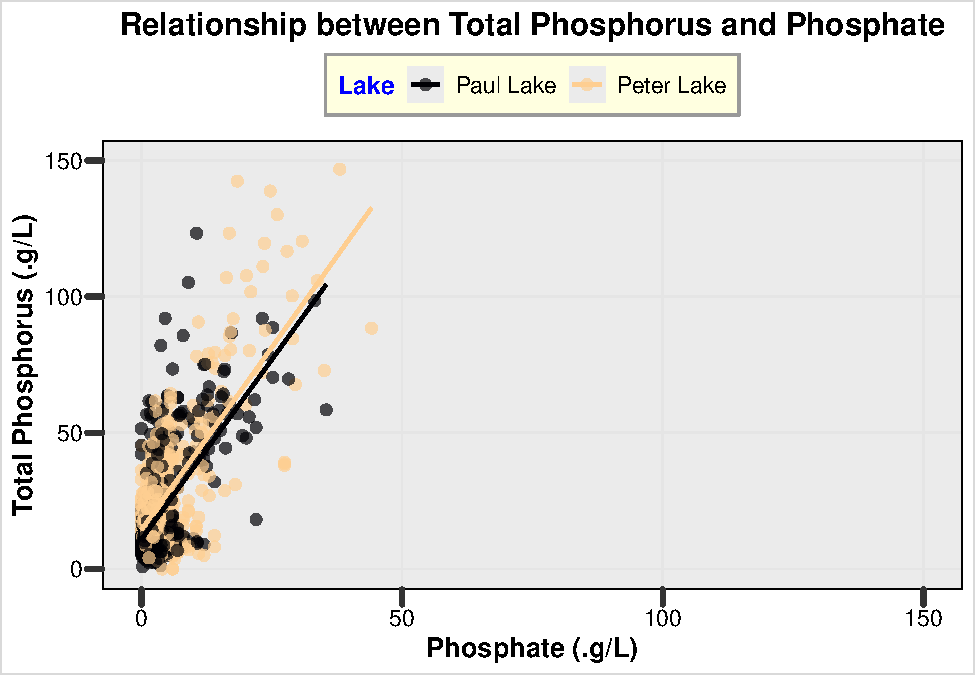
\includegraphics{Shuer-Li_A05_DataVisualization_files/figure-latex/plot total P vs PO4-1.pdf}

\begin{enumerate}
\def\labelenumi{\arabic{enumi}.}
\setcounter{enumi}{4}
\tightlist
\item
  {[}NTL-LTER{]} Make three separate boxplots of (a) temperature, (b)
  TP, and (c) TN, with month as the x axis and lake as a color
  aesthetic. Then, create a cowplot that combines the three graphs. Make
  sure that only one legend is present and that graph axes are aligned.
\end{enumerate}

Tips: * Recall the discussion on factors in the lab section as it may be
helpful here. * Setting an axis title in your theme to
\texttt{element\_blank()} removes the axis title (useful when multiple,
aligned plots use the same axis values) * Setting a legend's position to
``none'' will remove the legend from a plot. * Individual plots can have
different sizes when combined using \texttt{cowplot}.

\begin{Shaded}
\begin{Highlighting}[]
\CommentTok{\#5 Create separate boxplots of temperature, TP, and TN by month and lake, then combine with cowplot}
\FunctionTok{library}\NormalTok{(cowplot)}

\CommentTok{\# Convert month to factor for proper ordering}
\NormalTok{PeterPaul.chem.nutrients}\SpecialCharTok{$}\NormalTok{month }\OtherTok{\textless{}{-}} \FunctionTok{as.factor}\NormalTok{(PeterPaul.chem.nutrients}\SpecialCharTok{$}\NormalTok{month)}

\CommentTok{\# (a) Temperature}
\NormalTok{p\_temp }\OtherTok{\textless{}{-}} \FunctionTok{ggplot}\NormalTok{(PeterPaul.chem.nutrients,}
                 \FunctionTok{aes}\NormalTok{(}\AttributeTok{x =}\NormalTok{ month, }\AttributeTok{y =}\NormalTok{ temperature\_C, }\AttributeTok{color =}\NormalTok{ lakename)) }\SpecialCharTok{+}
  \FunctionTok{geom\_boxplot}\NormalTok{() }\SpecialCharTok{+}
  \FunctionTok{labs}\NormalTok{(}\AttributeTok{y =} \StringTok{"Temperature (°C)"}\NormalTok{, }\AttributeTok{x =} \StringTok{"Month"}\NormalTok{) }\SpecialCharTok{+}
  \FunctionTok{theme}\NormalTok{(}\AttributeTok{legend.position =} \StringTok{"none"}\NormalTok{)}

\CommentTok{\# (b) Total Phosphorus (TP)}
\NormalTok{p\_tp }\OtherTok{\textless{}{-}} \FunctionTok{ggplot}\NormalTok{(PeterPaul.chem.nutrients,}
               \FunctionTok{aes}\NormalTok{(}\AttributeTok{x =}\NormalTok{ month, }\AttributeTok{y =}\NormalTok{ tp\_ug, }\AttributeTok{color =}\NormalTok{ lakename)) }\SpecialCharTok{+}
  \FunctionTok{geom\_boxplot}\NormalTok{() }\SpecialCharTok{+}
  \FunctionTok{labs}\NormalTok{(}\AttributeTok{y =} \StringTok{"Total Phosphorus (μg/L)"}\NormalTok{, }\AttributeTok{x =} \StringTok{"Month"}\NormalTok{) }\SpecialCharTok{+}
  \FunctionTok{theme}\NormalTok{(}\AttributeTok{legend.position =} \StringTok{"none"}\NormalTok{)}

\CommentTok{\# (c) Total Nitrogen (TN)}
\NormalTok{p\_tn }\OtherTok{\textless{}{-}} \FunctionTok{ggplot}\NormalTok{(PeterPaul.chem.nutrients,}
               \FunctionTok{aes}\NormalTok{(}\AttributeTok{x =}\NormalTok{ month, }\AttributeTok{y =}\NormalTok{ tn\_ug, }\AttributeTok{color =}\NormalTok{ lakename)) }\SpecialCharTok{+}
  \FunctionTok{geom\_boxplot}\NormalTok{() }\SpecialCharTok{+}
  \FunctionTok{labs}\NormalTok{(}\AttributeTok{y =} \StringTok{"Total Nitrogen (μg/L)"}\NormalTok{, }\AttributeTok{x =} \StringTok{"Month"}\NormalTok{) }\SpecialCharTok{+}
  \FunctionTok{theme}\NormalTok{(}\AttributeTok{legend.position =} \StringTok{"top"}\NormalTok{)}

\CommentTok{\# Combine plots and align axes}
\FunctionTok{plot\_grid}\NormalTok{(p\_temp, p\_tp, p\_tn,}
          \AttributeTok{ncol =} \DecValTok{1}\NormalTok{, }\AttributeTok{align =} \StringTok{"v"}\NormalTok{)}
\end{Highlighting}
\end{Shaded}

\begin{verbatim}
## Warning: Removed 3566 rows containing non-finite outside the scale range
## (`stat_boxplot()`).
\end{verbatim}

\begin{verbatim}
## Warning: Removed 20729 rows containing non-finite outside the scale range
## (`stat_boxplot()`).
\end{verbatim}

\begin{verbatim}
## Warning: Removed 21583 rows containing non-finite outside the scale range
## (`stat_boxplot()`).
\end{verbatim}

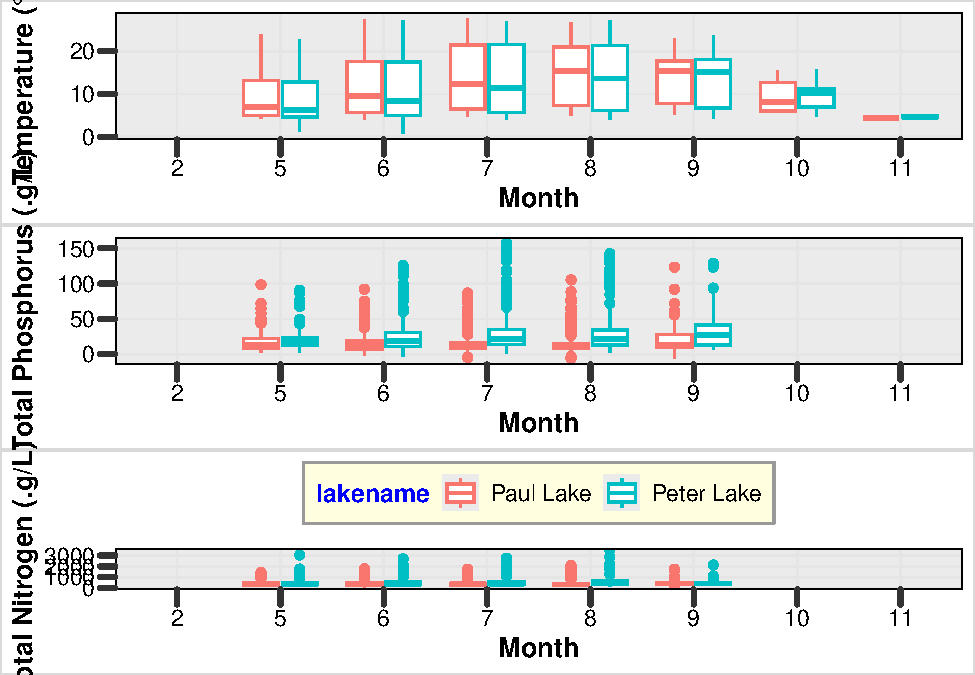
\includegraphics{Shuer-Li_A05_DataVisualization_files/figure-latex/Create boxplots-1.pdf}

Question: What do you observe about the variables of interest over
seasons and between lakes?

\begin{quote}
Answer: Temperature increases through the summer months and declines
toward autumn, showing a clear seasonal pattern. In contrast, total
phosphorus and total nitrogen vary less strongly with month but show
slightly higher concentrations in Peter Lake compared to Paul Lake
across most of the year. Overall, Peter Lake tends to have warmer and
more nutrient-rich conditions.
\end{quote}

\begin{enumerate}
\def\labelenumi{\arabic{enumi}.}
\setcounter{enumi}{5}
\item
  {[}Niwot Ridge{]} Plot a subset of the litter dataset by displaying
  only the ``Needles'' functional group. Plot the dry mass of needle
  litter by date and separate by NLCD class with a color aesthetic. (no
  need to adjust the name of each land use)
\item
  {[}Niwot Ridge{]} Now, plot the same plot but with NLCD classes
  separated into three facets rather than separated by color.
\end{enumerate}

\begin{Shaded}
\begin{Highlighting}[]
\CommentTok{\#6 Plot dry mass of needle litter by date, colored by NLCD class}
\NormalTok{Needles }\OtherTok{\textless{}{-}} \FunctionTok{subset}\NormalTok{(NIWO.litter, functionalGroup }\SpecialCharTok{==} \StringTok{"Needles"}\NormalTok{)}
\FunctionTok{ggplot}\NormalTok{(Needles, }\FunctionTok{aes}\NormalTok{(}\AttributeTok{x =}\NormalTok{ collectDate, }\AttributeTok{y =}\NormalTok{ dryMass, }\AttributeTok{color =}\NormalTok{ nlcdClass)) }\SpecialCharTok{+}
  \FunctionTok{geom\_point}\NormalTok{()}
\end{Highlighting}
\end{Shaded}

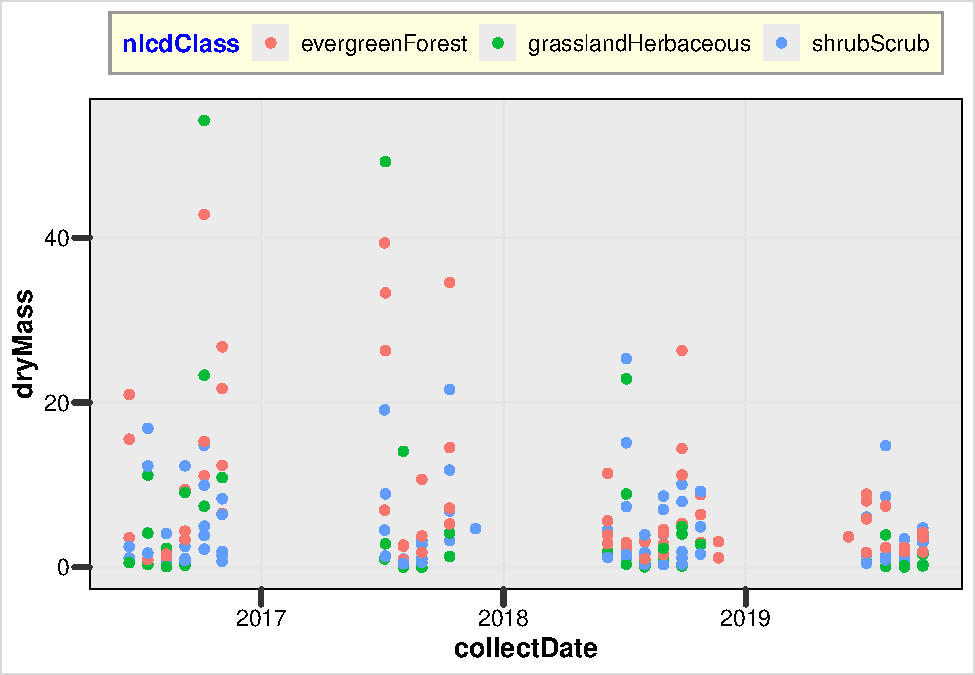
\includegraphics{Shuer-Li_A05_DataVisualization_files/figure-latex/Plot litter-1.pdf}

\begin{Shaded}
\begin{Highlighting}[]
\CommentTok{\#7 Plot dry mass of needle litter by date, faceted by NLCD class}
\FunctionTok{ggplot}\NormalTok{(Needles, }\FunctionTok{aes}\NormalTok{(}\AttributeTok{x =}\NormalTok{ collectDate, }\AttributeTok{y =}\NormalTok{ dryMass)) }\SpecialCharTok{+}
  \FunctionTok{geom\_point}\NormalTok{() }\SpecialCharTok{+}
  \FunctionTok{facet\_wrap}\NormalTok{(}\SpecialCharTok{\textasciitilde{}}\NormalTok{ nlcdClass)}
\end{Highlighting}
\end{Shaded}

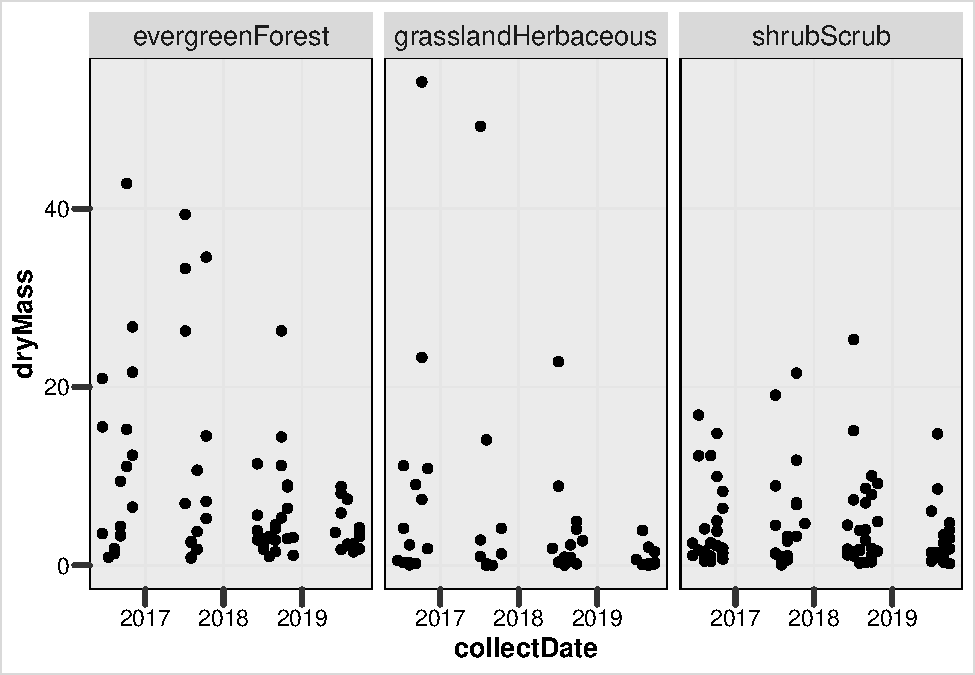
\includegraphics{Shuer-Li_A05_DataVisualization_files/figure-latex/Plot litter-2.pdf}
Question: Which of these plots (6 vs.~7) do you think is more effective,
and why?

\begin{quote}
Answer: The faceted plot (7) is more effective because it separates each
NLCD class into its own panel, making it easier to compare trends within
and between land-cover types without color overlap. In contrast, the
colored plot (6) is harder to interpret when points overlap across
classes.
\end{quote}

\end{document}
